\chapter{Correlaciones de Ising, campo medio y magnetización espontánea}

\lectureoverview{Una cadena de Ising unidimensional puede resolverse exactamente sustituyendo los espines de sitio por variables de enlace. Este cambio de variables convierte la función de partición en un producto y muestra que toda correlación a temperatura finita decae exponencialmente. Las redes de dimensiones superiores se comportan de otra manera porque cada espín recibe información de muchos vecinos. Si se trata su influencia conjunta como un campo promedio, se obtiene una ecuación de autoconsistencia, una temperatura crítica de campo medio y una descripción precisa de cómo un campo externo arbitrariamente pequeño selecciona una fase magnetizada.}

\section{Lo que Ising encontró realmente}

El punto histórico debe enunciarse con precisión. Ernst Ising resolvió el modelo unidimensional propuesto por Wilhelm Lenz y concluyó correctamente que no hay transición de fase a temperatura finita. La extrapolación excesiva consistió en inferir que la misma conclusión debía cumplirse en todas las dimensiones. No es así. El modelo bidimensional ya presenta una fase ordenada a baja temperatura.

Resolver exactamente el modelo en dimensiones superiores sería demasiado ambicioso para el propósito actual. Bastará una aproximación físicamente transparente para revelar la transición cuando cada espín tiene muchos vecinos. Sin embargo, antes de hacer esa aproximación, conviene resolver exactamente la cadena unidimensional. El contraste entre la solución exacta unidimensional y la aproximación de alta dimensión permite identificar el mecanismo que falta en una dimensión.

Aquí, una transición de fase significa algo más que un fortalecimiento gradual de una preferencia ya existente. Al cruzar la temperatura crítica, el estado de equilibrio adquiere una nueva propiedad macroscópica: puede persistir una magnetización distinta de cero incluso después de retirar el campo externo que se usó para orientar la muestra. Por tanto, el cálculo debe responder dos preguntas distintas. ¿Recuerda un espín lejano la orientación de un espín elegido? ¿Puede un campo infinitesimal organizar una muestra de tamaño arbitrario?

\section{El espín como elemento básico reutilizable}

Consideremos una variable de dos estados
\begin{equation}
\sigma=\pm1,
\end{equation}
y adoptemos la convención para la energía
\begin{equation}
E(\sigma)=-J\sigma,
\qquad J>0.
\end{equation}
El estado \(\sigma=+1\) tiene entonces menor energía. El parámetro \(J\) puede representar el producto de un momento magnético por un campo aplicado, pero en este cálculo solo interviene el producto.

Tratemos este espín como un subsistema pequeño en equilibrio térmico con todo lo demás. Su función de partición es
\begin{align}
z
&=\sum_{\sigma=\pm1}e^{-\beta E(\sigma)}
 =\sum_{\sigma=\pm1}e^{\beta J\sigma} \\
&=e^{\beta J}+e^{-\beta J}
 =2\cosh(\beta J).
\end{align}

El mismo resultado podría incorporarse a un conjunto de \(N\) espines independientes. La función de partición total sería simplemente \(Z=z^N\), de modo que \(\log Z=N\log z\) y cada magnitud termodinámica extensiva serían \(N\) veces su valor para un espín. Esta perspectiva de subsistema sustituye el recuento combinatorio más largo de cuántos espines apuntan hacia arriba y cuántos hacia abajo, pero contiene la misma información.
La energía promedio se obtiene a partir de la derivada logarítmica:
\begin{align}
\expect{E}
&=-\frac{\partial}{\partial\beta}\log z \\
&=-J\frac{\sinh(\beta J)}{\cosh(\beta J)}
 =-J\tanh(\beta J).
\end{align}
Como \(E=-J\sigma\),
\begin{equation}
\expect{\sigma}=\tanh(\beta J).
\end{equation}

\begin{figure}[ht]
\centering
\includegraphics[width=0.80\textwidth]{lecture_09_figure_02.png}
\caption{La energía y la magnetización de un espín, expresadas en términos de la tangente hiperbólica.}
\lectureframe{00:10:06}
\end{figure}

Esta fórmula reúne los dos límites de temperatura. A baja temperatura, \(\beta J\gg1\), y es casi seguro que el espín se encuentra en el estado de menor energía. A alta temperatura, \(\beta J\ll1\), por lo que
\begin{equation}
\expect{\sigma}\simeq \beta J\longrightarrow0.
\end{equation}
La agitación térmica borra el sesgo energético.

\begin{classroomqa}
\audiencequestion{¿Debe llevar signo negativo la energía promedio?}
\lecturerresponse{Sí. La identidad termodinámica es \(\expect{E}=-\partial_\beta\log z\), así que el resultado es \(-J\tanh(\beta J)\). Al dividir por el factor \(-J\) en \(E=-J\sigma\), se obtiene entonces la magnetización positiva \(\expect{\sigma}=\tanh(\beta J)\). \lecturetimestamp{00:09:15--00:09:44}}
\end{classroomqa}

\section{La cadena unidimensional}

Coloquemos \(N\) espines en una cadena abierta y hagamos que interactúen los espines vecinos:
\begin{equation}
H=-J\sum_{i=1}^{N-1}\sigma_i\sigma_{i+1},
\qquad \sigma_i=\pm1.
\label{eq:ising-chain}
\end{equation}
Para \(J>0\), un par paralelo aporta \(-J\), mientras que un par antiparalelo aporta \(+J\). Por tanto, los dos estados fundamentales son
\begin{equation}
(+,+,\ldots,+)
\qquad\text{and}\qquad
(-,-,\ldots,-).
\end{equation}

\begin{figure}[ht]
\centering
\includegraphics[width=0.80\textwidth]{lecture_09_figure_03.png}
\caption{El hamiltoniano de la cadena abierta y su suma de Boltzmann.}
\lectureframe{00:19:15}
\end{figure}

Cambiar \(J\) por \(-J\) favorece la alternancia de los espines. En una cadena abierta, o en una cadena periódica de longitud par, la redefinición
\begin{equation}
\widetilde{\sigma}_i=(-1)^i\sigma_i
\end{equation}
transforma el signo antiferromagnético en uno ferromagnético. La distinción es física, pero el álgebra de la función de partición unidimensional es la misma. La excepción conocida es una cadena periódica de longitud impar, que no puede alternar sin frustración.

\begin{classroomqa}
\audiencequestion{¿Hay un campo magnético externo en el hamiltoniano de la cadena?}
\lecturerresponse{Todavía no. La ecuación~\eqref{eq:ising-chain} solo contiene el acoplamiento entre primeros vecinos. Más adelante se añadirá por separado un campo externo uniforme, \(-h\sum_i\sigma_i\), precisamente para comprobar cómo responde el estado ordenado a un sesgo arbitrariamente pequeño. \lecturetimestamp{00:18:54--00:19:13}}
\end{classroomqa}

\subsection{La memoria como función de correlación}

Supongamos que se sabe que \(\sigma_i\) apunta hacia arriba. ¿Influye esa información en un espín situado a \(r\) enlaces de distancia? El diagnóstico es
\begin{equation}
C(r)=\expect{\sigma_i\sigma_{i+r}}.
\end{equation}
Si \(C(r)\) se aproxima a un valor distinto de cero cuando \(r\to\infty\), el sistema conserva memoria de largo alcance. Si se aproxima a cero, el efecto del primer espín acaba desapareciendo.

El juego del teléfono da la intuición adecuada. Cada persona transmite un símbolo binario a la siguiente. Si todas las transmisiones son perfectas, el bit inicial perdura indefinidamente. Si cada paso tiene una probabilidad de error distinta de cero, las transmisiones repetidas acaban perdiendo el mensaje original. La temperatura cero es el límite de transmisión perfecta de la cadena de Ising. Toda temperatura positiva permite desacuerdos ocasionales entre espines vecinos.

Para hacerse una idea numérica, supongamos que una transmisión tiene una fidelidad de \(0.99\). Dos transmisiones perfectas ocurren con probabilidad \(0.99^2=0.9801\), y cada paso adicional aporta otro factor \(0.99\). Tras cien pasos, los errores ya son comunes; tras diez mil, la memoria práctica se ha perdido. La cadena de Ising utiliza una medida de fidelidad con signo, en vez de la probabilidad de que no haya errores, pero la pérdida multiplicativa expresa la misma idea.

La analogía se vuelve exacta si se distingue entre probabilidad y correlación. Si \(p\) es la probabilidad de que dos espines adyacentes coincidan, entonces
\begin{equation}
\expect{\sigma_i\sigma_{i+1}}
=p-(1-p)=2p-1.
\end{equation}
Así, la cantidad que se multiplica de enlace en enlace es la fidelidad excedente \(2p-1\), no \(p\) propiamente dicha.

\section{Variables de enlace y función de partición exacta}

El cambio decisivo de variables consiste en describir las relaciones en lugar de los espines individuales:
\begin{equation}
\mu_i=\sigma_i\sigma_{i+1},
\qquad i=1,\ldots,N-1.
\label{eq:bond-variable}
\end{equation}
Cada variable de enlace vale \(+1\) si los espines coinciden y \(-1\) si discrepan. Si se fija el primer espín, los enlaces determinan todos los espines posteriores:
\begin{align}
\sigma_2&=\sigma_1\mu_1,\\
\sigma_3&=\sigma_1\mu_1\mu_2,\\
\sigma_{r+1}&=\sigma_1\prod_{k=1}^{r}\mu_k.
\end{align}
No hay redundancia. Los datos \((\sigma_1,\mu_1,\ldots,\mu_{N-1})\) son equivalentes a \((\sigma_1,\ldots,\sigma_N)\).

En estas variables, la energía es simplemente
\begin{equation}
H=-J\sum_{i=1}^{N-1}\mu_i.
\end{equation}
Las variables de sitio, que estaban acopladas, se han convertido en variables de enlace independientes. Al sumar primero sobre los dos valores de \(\sigma_1\) se obtiene
\begin{align}
Z_N
&=2\sum_{\{\mu_i=\pm1\}}
\exp\left(\beta J\sum_{i=1}^{N-1}\mu_i\right)\\
&=2\prod_{i=1}^{N-1}
\left(\sum_{\mu_i=\pm1}e^{\beta J\mu_i}\right)\\
&=2\left[2\cosh(\beta J)\right]^{N-1}.
\label{eq:chain-partition}
\end{align}
Hay \(N-1\) factores porque una cadena abierta de \(N\) sitios tiene \(N-1\) enlaces.

El factor inicial de dos corresponde a la elección global del primer espín. Solo aporta \(\log2\) a \(\log Z_N\), mientras que los enlaces aportan un término proporcional a \(N-1\). El factor importa para el recuento exacto de un sistema finito, pero desaparece de la densidad de energía libre cuando \(N\to\infty\). Por eso en la pizarra se podía decir que era «algo sin mayor importancia» sin descartarlo de verdad.

\begin{figure}[ht]
\centering
\includegraphics[width=0.82\textwidth]{lecture_09_figure_04.png}
\caption{El hamiltoniano de sitio reescrito como suma sobre enlaces independientes y la función de partición factorizada resultante.}
\lectureframe{00:35:35}
\end{figure}

\begin{classroomqa}
\audiencequestion{¿Adónde fue la suma del exponente cuando la respuesta final se convirtió en una potencia?}
\lecturerresponse{Primero se convirtió en un producto; después, en una potencia:
\[
e^{\beta J\sum_i\mu_i}=\prod_i e^{\beta J\mu_i}.
\]
La suma sobre todas las configuraciones de enlaces se separa entonces en una suma de dos términos por cada enlace. Como cada factor es \(2\cosh(\beta J)\), el producto es su potencia \((N-1)\). Al escribir explícitamente el caso de tres espines y dos enlaces, la factorización queda completamente clara. \lecturetimestamp{00:33:25--00:35:36}}
\end{classroomqa}

Esta es una descripción dual sencilla: las variables acopladas en los sitios se han sustituido por variables desacopladas en los enlaces. Es apropiado hablar de \emph{dualidad} porque el mismo sistema tiene dos descripciones con grados de libertad de aspecto muy distinto. Aquí se trata de un cambio exacto de variables para una cadena unidimensional abierta.

En el lenguaje de redes, las variables originales residen en los vértices y las nuevas, en las aristas. La elección global del primer espín es el dato adicional necesario para reconstruir los vértices a partir de las aristas. Este intercambio entre sitios y enlaces es un ejemplo modesto de un patrón que adquiere mucha más fuerza en la mecánica estadística de dimensiones superiores.

\subsection{Fidelidad entre primeros vecinos}

Todos los enlaces tienen la misma distribución,
\begin{equation}
\begin{aligned}
\Pr(\mu=+1)&=\frac{e^{\beta J}}{2\cosh(\beta J)},\\
\Pr(\mu=-1)&=\frac{e^{-\beta J}}{2\cosh(\beta J)}.
\end{aligned}
\end{equation}
Por consiguiente,
\begin{equation}
\expect{\mu_i}
=\expect{\sigma_i\sigma_{i+1}}
=\tanh(\beta J).
\label{eq:nearest-correlation}
\end{equation}

\begin{figure}[ht]
\centering
\includegraphics[width=0.80\textwidth]{lecture_09_figure_05.png}
\caption{La correlación entre primeros vecinos expresada como el valor medio de la variable de enlace.}
\lectureframe{00:36:52}
\end{figure}

Por tanto, la probabilidad de que los vecinos coincidan es
\begin{equation}
p_{\rm same}
=\frac{1+\tanh(\beta J)}{2}.
\end{equation}
Es mayor que un medio para \(J\) positivo, tiende a uno a temperatura cero y se convierte en un medio a temperatura infinita.

\begin{classroomqa}
\audiencequestion{¿Por qué una correlación positiva entre primeros vecinos significa que los espines prefieren alinearse en vez de antialinearse?}
\lecturerresponse{Para \(J>0\), un enlace alineado tiene energía \(-J\) y uno antialineado, energía \(+J\). El valor positivo de \(\expect{\mu}\) indica que \(\mu=+1\), es decir, la alineación, ocurre con mayor frecuencia. Que un material real tenga un acoplamiento efectivo ferro o antiferromagnético depende de su estructura electrónica microscópica; la convención de signos utilizada aquí describe un ferromagneto. \lecturetimestamp{00:43:45--00:44:48}}
\end{classroomqa}

\begin{classroomqa}
\audiencequestion{¿Qué ocurre con esta correlación a temperatura muy alta?}
\lecturerresponse{Cuando \(T\to\infty\), \(\beta\to0\) y \(\tanh(\beta J)\to0\). Entonces ni siquiera los vecinos más próximos llevan información unos de otros: cada espín equivale a una elección aleatoria. \lecturetimestamp{00:46:42--00:47:20}}
\end{classroomqa}

\subsection{Correlación a larga distancia}

Para espines separados por \(r\) enlaces,
\begin{align}
\sigma_i\sigma_{i+r}
&=\sigma_i
\left(\prod_{k=i+1}^{i+r-1}\sigma_k^2\right)
\sigma_{i+r}\\
&=(\sigma_i\sigma_{i+1})
(\sigma_{i+1}\sigma_{i+2})\cdots
(\sigma_{i+r-1}\sigma_{i+r})\\
&=\prod_{k=i}^{i+r-1}\mu_k.
\end{align}
Como las \(\mu_k\) son independientes,
\begin{equation}
C(r)=\expect{\sigma_i\sigma_{i+r}}
=\left[\tanh(\beta J)\right]^r.
\label{eq:exact-correlation}
\end{equation}

\begin{figure}[ht]
\centering
\includegraphics[width=0.80\textwidth]{lecture_09_figure_06.png}
\caption{Los factores intermedios \(\sigma_k^2=1\) convierten el producto de espines distantes en un producto de enlaces independientes.}
\lectureframe{00:41:35}
\end{figure}

\begin{classroomqa}
\audiencequestion{La función de correlación contiene solo los dos espines de los extremos. ¿De dónde salieron todos los espines intermedios?}
\lecturerresponse{Se introdujeron únicamente como factores iguales a uno: \(\sigma_k^2=1\). Agrupar las copias adyacentes convierte el producto de los extremos en variables de enlace, que son precisamente las variables cuya distribución térmica se factoriza. El valor de la función de correlación no ha cambiado. \lecturetimestamp{00:41:41--00:42:26}}
\end{classroomqa}

A toda temperatura finita,
\begin{equation}
0<\tanh(\beta J)<1,
\end{equation}
de modo que la memoria decae exponencialmente. Al escribir
\begin{equation}
C(r)=e^{-r/\xi}
\end{equation}
se define la longitud de correlación exacta
\begin{equation}
\xi^{-1}=-\log\!\left[\tanh(\beta J)\right].
\label{eq:correlation-length}
\end{equation}
Solo cuando \(T=0\) diverge \(\xi\). A baja temperatura, pero distinta de cero,
\begin{equation}
\xi\simeq \frac{1}{2}e^{2\beta J},
\end{equation}
por lo que la cadena puede contener tramos alineados muy largos sin tener orden verdadero de alcance infinito.

Por tanto, la cadena parece estar agrupada en bloques. Se observa un largo tramo de espines hacia arriba, luego un cambio, después un largo tramo de espines hacia abajo y, a continuación, otro cambio. A baja temperatura los tramos son largos porque las paredes de dominio son raras, pero no desaparecen del todo. La magnetización requiere una longitud de memoria infinita, no simplemente muy grande.

\section{Por qué tener más vecinos cambia el problema}

En una dimensión no hay corrección de errores. Cuando un enlace discrepa del anterior, el espín siguiente no tiene otra fuente independiente que le indique cuál era la orientación prevista. Por tanto, la cadena está formada por dominios largos y alineados, separados por cambios ocasionales.

En una red cuadrada, cada sitio tiene cuatro primeros vecinos. En una red cúbica, tiene seis. En una red hipercúbica de \(d\) dimensiones tiene
\begin{equation}
z=2d
\end{equation}
primeros vecinos. Un sitio que recibe tres mensajes concordantes y uno discordante puede seguir a la mayoría. Un entorno con muchos vecinos suprime los errores aislados de forma muy parecida a como los mensajes redundantes permiten corregir errores.

Si los vecinos tienen espín medio \(m\), su suma tiene media \(zm\). Su fluctuación habitual es del orden de \(\sqrt{z}\), de modo que, lejos de \(m=0\), la fluctuación relativa escala aproximadamente como
\begin{equation}
\frac{\sqrt{z}}{z|m|}
=\frac{1}{\sqrt{z}\,|m|}.
\end{equation}
Por eso un campo promedio resulta plausible cuando el número de coordinación es grande. También nos advierte de que la aproximación es menos fiable cerca de un punto crítico, donde \(m\) es pequeño.

Un dicho popular expresa la intuición de los grandes números: es poco probable que cien votos independientes se equivoquen en la misma dirección. La versión cuantitativa es la ley de la raíz cuadrada. El sesgo coherente de \(z\) variables es proporcional a \(z\), mientras que la discrepancia aleatoria suele ser proporcional solo a \(\sqrt{z}\). Así, al aumentar la dimensión, no solo cambia el número de vecinos, sino también la fiabilidad del mensaje colectivo que transmiten.

\begin{classroomqa}
\audiencequestion{¿Las dimensiones mayores que tres corresponden a un material magnético físico?}
\lecturerresponse{No como dimensiones espaciales directas. Un valor grande de \(d\) es un límite soluble en el que cada sitio tiene muchos vecinos y el promedio queda bajo control. Una vez que el mecanismo se hace visible en ese límite, se puede preguntar hasta qué punto persiste al acercarse a las dimensiones físicas. En el modelo de Ising, dos dimensiones ya bastan para que haya una transición a temperatura finita, aunque el campo medio no proporciona la respuesta bidimensional exacta. \lecturetimestamp{00:52:32--00:53:50}}
\end{classroomqa}

\section{El campo medio como problema de autoconsistencia}

Centremos la atención en un espín \(\sigma_i\). Su interacción con sus \(z=2d\) vecinos es
\begin{equation}
E_i=-J\sigma_i\sum_{j\in{\rm nn}(i)}\sigma_j.
\label{eq:local-energy}
\end{equation}
Sea
\begin{equation}
m=\expect{\sigma}
\end{equation}
la magnetización uniforme por espín. El campo medio sustituye la suma fluctuante de los espines vecinos por su promedio:
\begin{equation}
\sum_{j\in{\rm nn}(i)}\sigma_j
\longrightarrow zm=2dm.
\end{equation}
El espín elegido tiene entonces la energía efectiva de un espín
\begin{equation}
E_i^{\rm MF}=-2dJm\,\sigma_i.
\label{eq:mean-field-energy}
\end{equation}

\begin{figure}[ht]
\centering
\includegraphics[width=0.82\textwidth]{lecture_09_figure_07.png}
\caption{Un espín elegido, sus \(2d\) primeros vecinos y la sustitución de la suma de estos por la magnetización promedio.}
\lectureframe{01:00:30}
\end{figure}

Ahora se puede reutilizar el resultado para un espín con el campo efectivo \(2dJm\):
\begin{equation}
\expect{\sigma_i}_{\rm effective}
=\tanh(2\beta dJm).
\end{equation}
Pero el sitio elegido no tiene nada de especial. La invariancia traslacional exige que su promedio sea igual al promedio supuesto \(m\). Por tanto,
\begin{equation}
\boxed{m=\tanh(2\beta dJm)}.
\label{eq:self-consistency}
\end{equation}
Por eso el campo medio también se llama aproximación de campo autoconsistente: la magnetización que crea el campo efectivo debe ser igual a la magnetización producida por ese campo.

\begin{classroomqa}
\audiencequestion{¿Falta un factor de \(\beta\) en el resultado efectivo para un espín?}
\lecturerresponse{Debe estar presente. El argumento de una exponencial o de una tangente hiperbólica es adimensional, así que la energía efectiva \(2dJm\) aparece como \(2\beta dJm\). \lecturetimestamp{01:00:13--01:00:27}}
\end{classroomqa}

\begin{classroomqa}
\audiencequestion{¿La ecuación solo dice que \(m\) es proporcional a sí misma?}
\lecturerresponse{No. La magnetización desconocida aparece dentro de una función no lineal:
\[
m=\tanh(2\beta dJm).
\]
Es una ecuación implícita y puede tener una o varias soluciones, según la temperatura. \lecturetimestamp{01:02:12--01:02:42}}
\end{classroomqa}

\begin{classroomqa}
\audiencequestion{¿La ecuación de autoconsistencia supone una temperatura alta o un argumento pequeño de la tangente hiperbólica?}
\lecturerresponse{No. La ecuación \(m=\tanh(2\beta dJm)\) es la ecuación completa de campo medio a cualquier temperatura. Solo una aproximación posterior, como \(\tanh x\simeq x\), requiere que \(x\) sea pequeño; se utiliza cerca del punto crítico para localizar o desarrollar la solución emergente. \lecturetimestamp{01:02:44--01:03:12}}
\end{classroomqa}

\begin{classroomqa}
\audiencequestion{¿La notación con barra es distinta del promedio habitual entre corchetes angulares?}
\lecturerresponse{No. La barra que se usa en la pizarra es una abreviatura del promedio térmico: \(\bar{\sigma}=\expect{\sigma}=m\). \lecturetimestamp{01:03:19--01:03:42}}
\end{classroomqa}

\begin{classroomqa}
\audiencequestion{¿Son los espines \(2d\) todos primeros vecinos? ¿Tendrían un efecto parecido los acoplamientos de mayor alcance?}
\lecturerresponse{En una red hipercúbica, sí: hay dos primeros vecinos a lo largo de cada uno de los \(d\) ejes coordenados. Los acoplamientos a segundos vecinos y a distancias mayores corresponden a otro modelo y, por lo general, tienen sus propias intensidades; aun así, aumentar el alcance de la interacción también eleva el número de coordinación efectivo y puede hacer más preciso el razonamiento de campo medio. \lecturetimestamp{01:03:43--01:05:12}}
\end{classroomqa}

\section{Representación gráfica de la transición de fase}

Definamos
\begin{equation}
K=2\beta dJ,
\qquad
y=Km.
\end{equation}
Entonces, la ecuación~\eqref{eq:self-consistency} se convierte en
\begin{equation}
\frac{y}{K}=\tanh y.
\label{eq:graph-equation}
\end{equation}
El lado derecho es una función sigmoide fija. El lado izquierdo es una recta que pasa por el origen y cuya pendiente es
\begin{equation}
\frac{1}{K}=\frac{T}{2dJ},
\end{equation}
donde \(k_{\rm B}=1\).

A alta temperatura, la recta es muy inclinada y solo corta a \(\tanh y\) en \(y=0\). A baja temperatura, la recta es poco inclinada y hay tres intersecciones: \(y=0\) y un par simétrico \(y=\pm y_0\). El umbral se alcanza cuando la recta y \(\tanh y\) tienen la misma pendiente en el origen. Como \(\tanh'(0)=1\),
\begin{equation}
K_c=1,
\qquad
T_c^{\rm MF}=2dJ.
\label{eq:mean-field-tc}
\end{equation}
Esta es la temperatura crítica de campo medio, no la respuesta exacta en baja dimensión.

La hipótesis \(J>0\) indica que los espines vecinos prefieren coincidir; no selecciona \(+m\) frente a \(-m\). En ausencia de campo externo, el hamiltoniano no cambia bajo la inversión global \(\sigma_i\mapsto-\sigma_i\), de modo que las dos intersecciones distintas de cero son físicamente equivalentes. Dibujar solo la mitad positiva de la gráfica es una convención práctica, no una omisión de la fase negativa.

\begin{figure}[ht]
\centering
\includegraphics[width=0.82\textwidth]{lecture_09_figure_08.png}
\caption{La familia de rectas y \(\tanh y\): una sola intersección a alta temperatura y tres a baja temperatura.}
\lectureframe{01:11:50}
\end{figure}

\begin{figure}[ht]
\centering
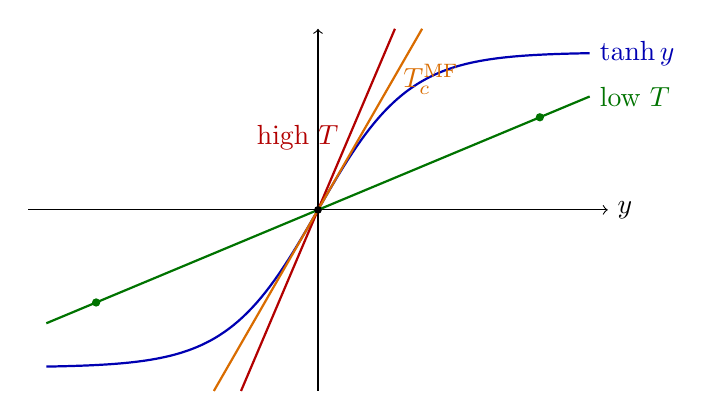
\begin{tikzpicture}[x=1.15cm,y=2.0cm]
\draw[->] (-3.2,0) -- (3.2,0) node[right] {$y$};
\draw[->] (0,-1.15) -- (0,1.15);
\draw[thick,blue!70!black,domain=-3:3,samples=120]
  plot (\x,{tanh(\x)}) node[right] {$\tanh y$};
\draw[thick,red!70!black] (-0.85,-1.15) -- (0.85,1.15)
  node[pos=0.70,left] {high \(T\)};
\draw[thick,orange!85!black] (-1.15,-1.15) -- (1.15,1.15)
  node[pos=0.86,right] {\(T_c^{\rm MF}\)};
\draw[thick,green!45!black] (-3,-0.72) -- (3,0.72)
  node[right] {low \(T\)};
\fill (0,0) circle (1.4pt);
\fill[green!45!black] (-2.45,-0.588) circle (1.5pt);
\fill[green!45!black] (2.45,0.588) circle (1.5pt);
\end{tikzpicture}
\caption{Reconstrucción normalizada del argumento gráfico de autoconsistencia.}
\end{figure}

La rama distinta de cero emerge de forma continua. Cerca de la transición,
\begin{equation}
\tanh(Km)=Km-\frac{(Km)^3}{3}+O(m^5).
\end{equation}
Para \(K>1\), las soluciones pequeñas distintas de cero satisfacen
\begin{equation}
m^2\simeq \frac{3(K-1)}{K^3}.
\end{equation}
Así, el campo medio predice la conocida aparición de raíz cuadrada \(m\propto(T_c-T)^{1/2}\).

La estabilidad también puede describirse sin depender de cómo se dibuje la gráfica. Salvo una constante independiente de \(m\), la energía libre de campo medio por espín es
\begin{equation}
f_{\rm MF}(m)
=dJm^2-\frac{1}{\beta}
\log\!\left[2\cosh(2\beta dJm)\right].
\label{eq:mf-free-energy}
\end{equation}
Su condición de estacionariedad es
\begin{equation}
\frac{\partial f_{\rm MF}}{\partial m}
=2dJ\left[m-\tanh(2\beta dJm)\right]=0.
\end{equation}
Por encima de \(T_c^{\rm MF}\), \(m=0\) es el mínimo. Por debajo, el origen es un máximo local y las dos soluciones distintas de cero son mínimos degenerados. La geometría de las intersecciones y la termodinámica de la energía libre conducen a la misma conclusión.

\begin{classroomqa}
\audiencequestion{La solución \(m=0\) sigue siendo una intersección por debajo de \(T_c^{\rm MF}\). ¿Por qué debería ser física la rama distinta de cero?}
\lecturerresponse{Si se sigue el sistema desde temperatura cero hacia arriba, ya se está en una rama magnetizada. Más formalmente, la energía libre de campo medio tiene mínimos en \(\pm m_0\) por debajo de la transición, mientras que \(m=0\) se convierte en un máximo. Un campo externo infinitesimal selecciona entonces uno de los mínimos y elimina la ambigüedad aparente. \lecturetimestamp{01:11:34--01:12:18}}
\end{classroomqa}

\section{Por qué la aproximación de campo medio falla en una dimensión}

Sustituir \(d=1\) en la ecuación~\eqref{eq:mean-field-tc} predeciría una transición en \(T=2J\), en contradicción con la solución unidimensional exacta. No hay ninguna singularidad algebraica. La aproximación falla porque dos vecinos no constituyen un gran baño estadístico y porque las paredes de dominio unidimensionales tienen una entropía excepcional.

Partamos del estado en que todos los espines apuntan hacia arriba. Un enlace roto cambia su energía de \(-J\) a \(+J\), de modo que cada enlace roto cuesta
\begin{equation}
\Delta E_{\rm bond}=2J.
\end{equation}
En una red cuadrada, invertir un espín rompe cuatro enlaces y cuesta \(8J\). Dos espines invertidos adyacentes tienen un perímetro de seis enlaces rotos y cuestan \(12J\), mientras que dos inversiones muy separadas rompen ocho enlaces y cuestan \(16J\).

\begin{figure}[ht]
\centering
\includegraphics[width=0.82\textwidth]{lecture_09_figure_09.png}
\caption{Dos espines invertidos adyacentes en una red cuadrada; su enlace compartido está satisfecho y queda un contorno de seis enlaces.}
\lectureframe{01:17:30}
\end{figure}

En dos dimensiones, por tanto, una gota compacta de espines invertidos paga una energía proporcional a la longitud de su contorno:
\begin{equation}
\Delta E_{\rm 2d}=2J\,|\partial D|.
\end{equation}
Al crecer la gota, por lo general también crece su contorno.

Una dimensión es distinta. Un bloque contiguo de espines invertidos, por largo que sea, solo tiene dos paredes de dominio:
\begin{equation}
\Delta E_{\rm 1d}=2(2J)=4J.
\label{eq:one-d-domain-cost}
\end{equation}

\begin{figure}[ht]
\centering
\includegraphics[width=0.82\textwidth]{lecture_09_figure_10.png}
\caption{Un bloque largo de espines invertidos en una dimensión, limitado por solo dos paredes de dominio.}
\lectureframe{01:19:10}
\end{figure}

Hay del orden de \(N^2\) maneras de elegir las dos paredes de ese bloque en una cadena de \(N\) sitios. Su energía no aumenta con la separación entre las paredes. A cualquier temperatura positiva, la entropía permite entonces dominios invertidos de tamaño arbitrario. En dos dimensiones, a temperatura suficientemente baja, la energía del contorno puede superar la entropía de los contornos. Esta competencia entre energía y entropía es el hecho geométrico que el campo medio no puede captar cuando trata \(d=1\) y \(d=2\) como simples valores numéricos distintos del mismo coeficiente.

\begin{classroomqa}
\audiencequestion{¿El coste constante de dos paredes exige que los espines invertidos sean adyacentes?}
\lecturerresponse{Sí. La afirmación se refiere a un único bloque contiguo de espines invertidos. Si forman varios bloques separados, cada bloque introduce dos paredes de dominio adicionales. Lo importante es que un único bloque puede tener longitud arbitraria y conservar solo dos paredes. \lecturetimestamp{01:18:32--01:18:40}}
\end{classroomqa}

\begin{classroomqa}
\audiencequestion{La propia ecuación de campo medio no parece distinguir cualitativamente entre \(d=1\) y \(d=2\). ¿Ese es el problema?}
\lecturerresponse{Exactamente. El campo medio predice una transición para todo \(d\) positivo, así que es cualitativamente erróneo en una dimensión. Su derivación supuso muchos vecinos con fluctuaciones débiles y descartó la geometría de las paredes de dominio. El caso unidimensional lo determina la solución exacta en variables de enlace, no la sustitución de campo medio \(d=1\). \lecturetimestamp{01:19:44--01:20:28}}
\end{classroomqa}

\section{Un campo externo selecciona la fase}

Añadamos un campo uniforme \(h\), con la convención de que \(h>0\) favorece \(\sigma=+1\):
\begin{equation}
H=-J\sum_{\langle ij\rangle}\sigma_i\sigma_j
-h\sum_i\sigma_i.
\label{eq:ising-with-field}
\end{equation}
La energía de campo medio de un espín elegido es
\begin{equation}
E_i^{\rm MF}=-(2dJm+h)\sigma_i,
\end{equation}
y la ecuación de autoconsistencia se convierte en
\begin{equation}
\boxed{m=\tanh\!\left[\beta(2dJm+h)\right]}.
\label{eq:self-consistency-field}
\end{equation}
Con \(K=2\beta dJ\) y \(y=Km\),
\begin{equation}
\frac{y}{K}=\tanh(y+\beta h).
\label{eq:shifted-graph}
\end{equation}

\begin{figure}[ht]
\centering
\includegraphics[width=0.82\textwidth]{lecture_09_figure_11.png}
\caption{El término de campo externo añadido a la ecuación de autoconsistencia, junto con la construcción gráfica desplazada.}
\lectureframe{01:26:20}
\end{figure}

\begin{classroomqa}
\audiencequestion{¿Por qué se añade el campo solo dentro de la tangente hiperbólica? ¿No debería modificar también el lado izquierdo?}
\lecturerresponse{El lado izquierdo es la magnetización supuesta \(m\), o, de manera equivalente, \(y/K\). El lado derecho es la magnetización calculada para un espín en el campo efectivo total \(2dJm+h\). La autoconsistencia iguala esas dos cantidades. Mantener \(y=Km\) fijo como definición hace que el término nuevo aparezca solo en el argumento \(\tanh(y+\beta h)\). \lecturetimestamp{01:23:46--01:26:18}}
\end{classroomqa}

\begin{classroomqa}
\audiencequestion{¿Puede describirse el mismo cambio gráfico desplazando las rectas en vez de desplazar la curva \(\tanh\)?}
\lecturerresponse{Sí. Se puede mantener \(\tanh y\) fijo y reescribir la ecuación de modo que la recta tenga una ordenada en el origen distinta de cero. Las intersecciones son idénticas. Las dos descripciones solo difieren en qué lado de la ecuación se toma como gráfica fija. \lecturetimestamp{01:35:07--01:36:26}}
\end{classroomqa}

Para \(h\neq0\), el origen ya no es una solución. Por debajo de \(T_c^{\rm MF}\), un campo positivo arbitrariamente pequeño selecciona la rama positiva; un campo negativo selecciona la negativa.

\begin{figure}[ht]
\centering
\includegraphics[width=0.82\textwidth]{lecture_09_figure_12.png}
\caption{Un campo débil elimina la intersección simétrica y selecciona una de las ramas magnetizadas.}
\lectureframe{01:36:22}
\end{figure}

El enunciado correcto exige especificar el orden de los límites. Un sistema finito exactamente a \(h=0\) tiene simetría de inversión de espín y, por tanto, \(\expect{m}=0\) en el conjunto de equilibrio completo. La magnetización espontánea es
\begin{equation}
m_{\rm sp}
=\lim_{h\to0^+}\lim_{N\to\infty}\expect{m}_{N,h},
\end{equation}
tomando primero el límite termodinámico. Si se invierte el signo del campo infinitesimal, se obtiene \(-m_{\rm sp}\). La diferencia de energía debida al campo total es proporcional a \(Nh\), de modo que incluso un campo minúsculo se vuelve decisivo para una muestra macroscópica.

La energía libre correspondiente hace visible la inclinación:
\begin{equation}
f_{\rm MF}(m;h)
=dJm^2-\frac{1}{\beta}
\log\!\left[2\cosh\!\left(\beta(2dJm+h)\right)\right].
\end{equation}
Para \(h=0\), los dos pozos tienen la misma profundidad. Un valor positivo de \(h\) baja el pozo de \(m\) positivo y sube el de \(m\) negativo. La perturbación por espín puede ser minúscula, mientras que la preferencia total, multiplicada por \(N\), es macroscópica.

\begin{classroomqa}
\audiencequestion{Si el campo externo sigue presente, ¿la magnetización es realmente espontánea?}
\lecturerresponse{El campo solo se utiliza para seleccionar una rama. A temperatura fija \(T<T_c\), se lleva el sistema al límite de tamaño infinito y luego se hace \(h\to0^+\). La magnetización sigue siendo finita aunque el campo selector se anule. Si se invierte el signo en el límite, se selecciona la fase opuesta. \lecturetimestamp{01:33:15--01:34:18}}
\end{classroomqa}

\begin{classroomqa}
\audiencequestion{¿La solución de promedio cero es realmente imposible por debajo de la transición, o simplemente es inestable?}
\lecturerresponse{Con campo exactamente nulo, es posible tener un conjunto de volumen finito simétrico, con igual peso para las dos orientaciones y promedio cero. Lo que deja de ser estable es que constituya una única fase macroscópica. Un campo arbitrariamente pequeño altera el balance de energía extensiva y selecciona una orientación; tras tomar el límite termodinámico, la magnetización seleccionada persiste al retirar el campo. \lecturetimestamp{01:34:25--01:35:06}}
\end{classroomqa}

\begin{classroomqa}
\audiencequestion{¿Qué ocurre con la solución sesgada por el campo a temperatura infinita?}
\lecturerresponse{Para un valor fijo y finito de \(h\), tanto \(K=2\beta dJ\) como \(\beta h\) se anulan cuando \(T\to\infty\). La ecuación~\eqref{eq:self-consistency-field} da entonces \(m\to0\). El campo débil selecciona una rama de baja temperatura, pero no puede mantener el orden frente a la agitación térmica infinita. \lecturetimestamp{01:27:39--01:29:51}}
\end{classroomqa}

\begin{classroomqa}
\audiencequestion{Cuando varían a la vez la temperatura y el desplazamiento de la gráfica, ¿cómo se puede saber hacia dónde se mueve la intersección?}
\lecturerresponse{La ecuación implícita es más fiable que el esquema móvil. A baja temperatura y con \(h\) positivo, su solución estable se aproxima a \(m=+1\). A alta temperatura, al desarrollar la tangente se obtiene
\[
m\simeq \beta(2dJm+h)
\quad\Longrightarrow\quad
m\simeq \frac{\beta h}{1-2\beta dJ},
\]
que tiende a cero cuando \(\beta\to0\). Por tanto, la rama estable conecta el límite alineado de baja temperatura con el límite débilmente polarizado de alta temperatura, sin permanecer en el origen inestable por debajo de la transición. \lecturetimestamp{01:29:53--01:33:04}}
\end{classroomqa}

\section{La inversión del campo magnético plantea un problema distinto}

\begin{classroomqa}
\audiencequestion{¿Qué hace que el campo magnético terrestre invierta su dirección?}
\lecturerresponse{Esa pregunta queda fuera del modelo de Ising en equilibrio. El campo principal de la Tierra se genera mediante la geodinamo: la convección y la rotación del fluido eléctricamente conductor del núcleo externo mantienen las corrientes eléctricas y el campo magnético. Las inversiones son reorganizaciones irregulares de esa dinamo no lineal, no un simple cambio de orientación de dominios ferromagnéticos en hierro sólido. Su cronología detallada no puede describirse mediante un único parámetro de orden de equilibrio; por eso, la respuesta honesta aquí es que el cálculo de Ising no explica qué las desencadena. La conexión útil es solo la general: un sistema con dos orientaciones opuestas a gran escala puede sufrir una inestabilidad que lo haga pasar de una a otra.\footnote{Consúltese la \href{https://science.nasa.gov/science-research/earth-science/earths-magnetosphere-protecting-our-planet-from-harmful-space-energy/}{descripción general de la NASA sobre la geodinamo} y la \href{https://www.usgs.gov/programs/geomagnetism/introduction-geomagnetism}{introducción del USGS al geomagnetismo}.} \lecturetimestamp{01:38:39--01:40:32}}
\end{classroomqa}

La cadena exacta y la red de campo medio dan ahora dos respuestas claramente distintas. En una dimensión,
\begin{equation}
\expect{\sigma_i\sigma_{i+r}}
=\left[\tanh(\beta J)\right]^r
\longrightarrow0
\qquad (T>0),
\end{equation}
pues las paredes de dominio de energía finita pueden separar intervalos invertidos de longitud arbitraria. Con muchos vecinos, en cambio, el campo autoconsistente admite soluciones estables no nulas por debajo de
\begin{equation}
T_c^{\rm MF}=2dJ.
\end{equation}
La diferencia no es meramente algebraica. Se debe a la competencia entre geometría, energía, entropía y redundancia: si un error puede propagarse libremente o si la red circundante puede corregirlo.